\usepackage{ifthen}
\usepackage{tikz}
\usepackage{pgf}
\usepackage{pgffor}
\usepgfmodule{shapes}
\usepgfmodule{plot}
\usetikzlibrary{decorations}
\usetikzlibrary{arrows}
\usetikzlibrary{snakes}
\usetikzlibrary{calc}
\usetikzlibrary{positioning}

\newcommand{\PlotGrid}[4]{
	\draw[very thin,color=gray, dotted] (#1,#3) grid (#2,#4);
}
\newcommand{\PlotAxes}[6]{
	\draw[->, >=latex] (#1,0) -- (#2,0) node[right] {#5};
	\draw[->, >=latex] (0,#3) -- (0,#4) node[right] {#6};
}
\newcommand{\PlotAxesWithoutLabels}[5]{
	\draw[-] (#1,0) -- (#2,0);
	\draw[-] (#5,#3) -- (#5,#4);
	
}
\newcommand{\ZeigerdiagrammText}[4]{
	\begin{tikzpicture}[scale=.72, samples=100, >=latex]
	
	\def\Theta{#1}
	\def\Phase{#2}
	\def\VoltageMagnitude{#3}
	\def\CurrentMagnitude{#4}
	\def\SpannungsWert{{\VoltageMagnitude*sin(\Theta)}}
	\def\StromWert{{\CurrentMagnitude*sin(\Theta+\Phase)}}
	%%%%%%%%%%%%%%%%%%%%%%%%%%%%%%%%%%%%%%%%%%%%%%%%%%%%%%%%%%
	\def\VoltageColor{blue!90!white}
	\def\CurrentColor{red!90!white}
	\def\FarbeWinkelZeichnung{green}
	%%%%%%%%%%%%%%%%%%%%%%%%%%%%%%%%%%%%%%%%%%%%%%%%%%%%%%%%%%
	\def\Beta{\Theta+\Phase}
	\def\ThetaRad{\Theta*3.141592654/180}
	\def\PhaseRad{\Phase*3.141592654/180}
	%%%%%%%%%%%%%%%%%%%%%%%%%%%%%%%%%%%%%%%%%%%%%%%%%%%%%%%%%%
	\PlotGrid{-.1}{7.1}{-3.1}{3.1}
	\PlotAxes{-.2}{7.3}{-3.2}{3.3}{$\omega t$}{}
	\draw (1.570795,0) node[below]{$\frac{\pi}{2}$};
	\draw (3.14159,0) node[below]{${\pi}$};
	\draw (4.71238898,0) node[below]{$\frac{3\pi}{2}$};
	\draw (6.283185307,0) node[below]{${2\pi}$};
	\draw (-4,0) circle (3cm);
	\PlotAxesWithoutLabels{-7.2}{-.8}{-3.6}{3.6}{-4}
	%%%%%%%%%%%%%%%%%%%%%%%%%%%%%%%%%%%%%%%%%%%%%%%%%%%%%%%%%%
	
	% voltage
	\draw[color=\VoltageColor, very thick] plot[id=voltage, domain=0:7] function{\VoltageMagnitude*cos(x+\ThetaRad)} node[right] {$v(t)/\sqrt{2}$};
	% voltage circle
	\draw[color=\VoltageColor, loosely dashed] (-4,0) circle (\VoltageMagnitude cm);
	% angle
	%\draw[color=\FarbeWinkelZeichnung!50!black, thick] (\ThetaRad, \SpannungsWert)--(\ThetaRad,\StromWert) node[below=18pt] {$\theta$};
	% angle in the circle
	\filldraw[fill=\FarbeWinkelZeichnung!20,draw=\FarbeWinkelZeichnung!50!black] (-4,0) node[above=5pt] {$\phi$} -- (-4+0.866,0.5) arc (\Theta:\Beta:1) -- cycle ;
	% voltage pointer
	\draw[<-,color=\VoltageColor, very thick] (\Theta:\VoltageMagnitude)++(-4,0) --(-4,0);
	%\draw[color=\VoltageColor,  dashed] (\Theta:\VoltageMagnitude)++(-4,0) -- (\ThetaRad,\SpannungsWert);
	% current
	\draw[color=\CurrentColor, very thick] plot[id=current, domain=0:7] function{\CurrentMagnitude*cos(x+\PhaseRad+\ThetaRad)} node[right] {$i(t)/\sqrt{2}$};		
	% current circle
	\draw[color=\CurrentColor, loosely dashed]    (-4,0) circle (\CurrentMagnitude cm);
	% current pointer
	\draw[<-,color=\CurrentColor, very thick] (\Beta:\CurrentMagnitude)++(-4,0) --(-4,0);
	% angular velocity \omega
	\draw[->, xshift=-4cm]  (120:2.4cm) arc (120:170:2) node[below] {$\omega$};
	\end{tikzpicture}
}

\newcommand{\TimeDiagram}[4]{
	\begin{tikzpicture}[scale=.62, samples=100, >=latex]
	
	\def\Theta{#1}
	\def\Phase{#2}
	\def\VoltageMagnitude{#3}
	\def\CurrentMagnitude{#4}
	\def\SpannungsWert{{\VoltageMagnitude*sin(\Theta)}}
	\def\StromWert{{\CurrentMagnitude*sin(\Theta+\Phase)}}
	%%%%%%%%%%%%%%%%%%%%%%%%%%%%%%%%%%%%%%%%%%%%%%%%%%%%%%%%%%
	\def\VoltageColor{blue!90!white}
	\def\CurrentColor{red!90!white}
	\def\FarbeWinkelZeichnung{green}
	%%%%%%%%%%%%%%%%%%%%%%%%%%%%%%%%%%%%%%%%%%%%%%%%%%%%%%%%%%
	\def\Beta{\Theta+\Phase}
	\def\ThetaRad{\Theta*3.141592654/180}
	\def\PhaseRad{\Phase*3.141592654/180}
	%%%%%%%%%%%%%%%%%%%%%%%%%%%%%%%%%%%%%%%%%%%%%%%%%%%%%%%%%%
	\PlotGrid{-.1}{7.1}{-3.1}{3.1}
	\PlotAxes{-.2}{7.3}{-3.2}{3.3}{$\omega t$}{}
	\draw (1.570795,0) node[below]{$\frac{\pi}{2}$};
	\draw (3.14159,0) node[below]{${\pi}$};
	\draw (4.71238898,0) node[below]{$\frac{3\pi}{2}$};
	\draw (6.283185307,0) node[below]{${2\pi}$};
	%%%%%%%%%%%%%%%%%%%%%%%%%%%%%%%%%%%%%%%%%%%%%%%%%%%%%%%%%%
	
	% voltage
	\draw[-, color=\VoltageColor, dotted, thick] (-2, \VoltageMagnitude) to (7, \VoltageMagnitude);
	\draw[<->, color=\VoltageColor, thick] (-2, 0) to node[left]{$\sqrt{2} V$} (-2, \VoltageMagnitude);
	\draw[color=\VoltageColor, very thick] plot[id=voltageTime, domain=0:7] function{\VoltageMagnitude*cos(x+\ThetaRad)} node[right] {$v(t)$};
	% angle
	%\draw[color=\FarbeWinkelZeichnung!50!black, thick] (\ThetaRad, \SpannungsWert)--(\ThetaRad,\StromWert) node[below=18pt] {$\theta$};
	% current
	\draw[-, color=\CurrentColor, dotted, thick] (-.5, \CurrentMagnitude) to (7, \CurrentMagnitude);
	\draw[<->, color=\CurrentColor, thick] (-.5, 0) to node[left]{$\sqrt{2} I$} (-.5, \CurrentMagnitude);
	\draw[color=\CurrentColor, very thick] plot[id=currentTime, domain=0:7] function{\CurrentMagnitude*cos(x+\ThetaRad\PhaseRad)} node[right] {$i(t)$};		
	\end{tikzpicture}
}

\newcommand{\PowerTimeDiagram}[3]{
	\begin{tikzpicture}[scale=.5, samples=100, >=latex]
	\def\Phi{#1}
	\def\PhiRad{\Phi*3.141592654/180}
	\def\VoltageMagnitude{#2}
	\def\CurrentMagnitude{#3}
	\def\ActivePower{\VoltageMagnitude*\CurrentMagnitude*cos(\PhiRad)}
	\def\ReactivePower{\VoltageMagnitude*\CurrentMagnitude*sin(\PhiRad)}
	%%%%%%%%%%%%%%%%%%%%%%%%%%%%%%%%%%%%%%%%%%%%%%%%%%%%%%%%%%
	\def\VoltageColor{blue!90!white}
	\def\CurrentColor{red!90!white}
	\def\FarbeWinkelZeichnung{green!50!black}
	%%%%%%%%%%%%%%%%%%%%%%%%%%%%%%%%%%%%%%%%%%%%%%%%%%%%%%%%%%
	\PlotGrid{-.1}{7.1}{-3.1}{3.1}
	\PlotAxes{-.2}{7.3}{-3.2}{3.3}{$\omega t$}{}
	\draw (1.570795,0) node[below]{$\frac{\pi}{2}$};
	\draw (3.14159,0) node[below]{${\pi}$};
	\draw (4.71238898,0) node[below]{$\frac{3\pi}{2}$};
	\draw (6.283185307,0) node[below]{${2\pi}$};
	%%%%%%%%%%%%%%%%%%%%%%%%%%%%%%%%%%%%%%%%%%%%%%%%%%%%%%%%%%
	
	% voltage
	\draw[color=\VoltageColor] plot[id=voltageTimeP, domain=0:7] function{\VoltageMagnitude*cos(x+\PhiRad)} node[right] {$v(t)$};
	% current
	\draw[color=\CurrentColor] plot[id=currentTimeP, domain=0:7] function{\CurrentMagnitude*cos(x)} node[right] {$i(t)$};		
	% power
	\draw[color=\FarbeWinkelZeichnung, thick, dotted] plot[id=activePowerP, domain=0:7] function{\ActivePower} ;
	\draw[color=\FarbeWinkelZeichnung, very thick] plot[id=powerTimeP, domain=0:7] function{\ActivePower +\ActivePower*cos(2*x)-\ReactivePower*sin(2*x)} node[above=20pt, right] {$p(t)$};
	\end{tikzpicture}
}


\newcommand{\PowerTimeDiagramR}[2]{
	\begin{tikzpicture}[scale=.3, samples=100, >=latex]
	\def\Phi{0}
	\def\PhiRad{\Phi*3.141592654/180}
	\def\VoltageMagnitude{#1}
	\def\CurrentMagnitude{#2}
	\def\ActivePower{\VoltageMagnitude*\CurrentMagnitude*cos(\PhiRad)}
	\def\ReactivePower{\VoltageMagnitude*\CurrentMagnitude*sin(\PhiRad)}
	%%%%%%%%%%%%%%%%%%%%%%%%%%%%%%%%%%%%%%%%%%%%%%%%%%%%%%%%%%
	\def\VoltageColor{blue!90!white}
	\def\CurrentColor{red!90!white}
	\def\FarbeWinkelZeichnung{green!50!black}
	%%%%%%%%%%%%%%%%%%%%%%%%%%%%%%%%%%%%%%%%%%%%%%%%%%%%%%%%%%
	\PlotGrid{-.1}{7.1}{-3.1}{3.1}
	\PlotAxes{-.2}{7.3}{-3.2}{3.3}{$\omega t$}{}
	\draw (1.570795,0) node[below]{$\frac{\pi}{2}$};
	\draw (3.14159,0) node[below]{${\pi}$};
	\draw (4.71238898,0) node[below]{$\frac{3\pi}{2}$};
	\draw (6.283185307,0) node[below]{${2\pi}$};
	%%%%%%%%%%%%%%%%%%%%%%%%%%%%%%%%%%%%%%%%%%%%%%%%%%%%%%%%%%
	
	% voltage
	\draw[color=\VoltageColor] plot[id=voltageTimeR, domain=0:7] function{\VoltageMagnitude*cos(x+\PhiRad)} node[right] {};
	% current
	\draw[color=\CurrentColor] plot[id=currentTimeR, domain=0:7] function{\CurrentMagnitude*cos(x)} node[right] {};		
	% power
	\draw[color=\FarbeWinkelZeichnung, thick, dotted] plot[id=activePowerR, domain=0:7] function{\ActivePower} ;
	\draw[color=\FarbeWinkelZeichnung, very thick] plot[id=powerTimeR, domain=0:7] function{\ActivePower +\ActivePower*cos(2*x)-\ReactivePower*sin(2*x)} node[above=20pt, right] {};
	\end{tikzpicture}
}

\newcommand{\PowerTimeDiagramL}[2]{
	\begin{tikzpicture}[scale=.3, samples=100, >=latex]
	\def\Phi{90}
	\def\PhiRad{\Phi*3.141592654/180}
	\def\VoltageMagnitude{#1}
	\def\CurrentMagnitude{#2}
	\def\ActivePower{\VoltageMagnitude*\CurrentMagnitude*cos(\PhiRad)}
	\def\ReactivePower{\VoltageMagnitude*\CurrentMagnitude*sin(\PhiRad)}
	%%%%%%%%%%%%%%%%%%%%%%%%%%%%%%%%%%%%%%%%%%%%%%%%%%%%%%%%%%
	\def\VoltageColor{blue!90!white}
	\def\CurrentColor{red!90!white}
	\def\FarbeWinkelZeichnung{green!50!black}
	%%%%%%%%%%%%%%%%%%%%%%%%%%%%%%%%%%%%%%%%%%%%%%%%%%%%%%%%%%
	\PlotGrid{-.1}{7.1}{-3.1}{3.1}
	\PlotAxes{-.2}{7.3}{-3.2}{3.3}{$\omega t$}{}
	\draw (1.570795,0) node[below]{$\frac{\pi}{2}$};
	\draw (3.14159,0) node[below]{${\pi}$};
	\draw (4.71238898,0) node[below]{$\frac{3\pi}{2}$};
	\draw (6.283185307,0) node[below]{${2\pi}$};
	%%%%%%%%%%%%%%%%%%%%%%%%%%%%%%%%%%%%%%%%%%%%%%%%%%%%%%%%%%
	
	% voltage
	\draw[color=\VoltageColor] plot[id=voltageTimeL, domain=0:7] function{\VoltageMagnitude*cos(x+\PhiRad)} node[right] {};
	% current
	\draw[color=\CurrentColor] plot[id=currentTimeL, domain=0:7] function{\CurrentMagnitude*cos(x)} node[right] {};		
	% power
	\draw[color=\FarbeWinkelZeichnung, thick, dotted] plot[id=activePowerL, domain=0:7] function{\ActivePower} ;
	\draw[color=\FarbeWinkelZeichnung, very thick] plot[id=powerTimeL, domain=0:7] function{\ActivePower +\ActivePower*cos(2*x)-\ReactivePower*sin(2*x)} node[above=20pt, right] {};
	\end{tikzpicture}
}

\newcommand{\PowerTimeDiagramC}[2]{
	\begin{tikzpicture}[scale=.3, samples=100, >=latex]
	\def\Phi{-90}
	\def\PhiRad{\Phi*3.141592654/180}
	\def\VoltageMagnitude{#1}
	\def\CurrentMagnitude{#2}
	\def\ActivePower{\VoltageMagnitude*\CurrentMagnitude*cos(\PhiRad)}
	\def\ReactivePower{\VoltageMagnitude*\CurrentMagnitude*sin(\PhiRad)}
	%%%%%%%%%%%%%%%%%%%%%%%%%%%%%%%%%%%%%%%%%%%%%%%%%%%%%%%%%%
	\def\VoltageColor{blue!90!white}
	\def\CurrentColor{red!90!white}
	\def\FarbeWinkelZeichnung{green!50!black}
	%%%%%%%%%%%%%%%%%%%%%%%%%%%%%%%%%%%%%%%%%%%%%%%%%%%%%%%%%%
	\PlotGrid{-.1}{7.1}{-3.1}{3.1}
	\PlotAxes{-.2}{7.3}{-3.2}{3.3}{$\omega t$}{}
	\draw (1.570795,0) node[below]{$\frac{\pi}{2}$};
	\draw (3.14159,0) node[below]{${\pi}$};
	\draw (4.71238898,0) node[below]{$\frac{3\pi}{2}$};
	\draw (6.283185307,0) node[below]{${2\pi}$};
	%%%%%%%%%%%%%%%%%%%%%%%%%%%%%%%%%%%%%%%%%%%%%%%%%%%%%%%%%%
	
	% voltage
	\draw[color=\VoltageColor] plot[id=voltageTimeC, domain=0:7] function{\VoltageMagnitude*cos(x+\PhiRad)} node[right] {};
	% current
	\draw[color=\CurrentColor] plot[id=currentTimeC, domain=0:7] function{\CurrentMagnitude*cos(x)} node[right] {};		
	% power
	\draw[color=\FarbeWinkelZeichnung, thick, dotted] plot[id=activePowerC, domain=0:7] function{\ActivePower} ;
	\draw[color=\FarbeWinkelZeichnung, very thick] plot[id=powerTimeC, domain=0:7] function{\ActivePower +\ActivePower*cos(2*x)-\ReactivePower*sin(2*x)} node[above=20pt, right] {};
	\end{tikzpicture}
}

\newcommand{\RMS}[1]{
	\begin{tikzpicture}[scale=.72, samples=100, >=latex]
	
	\def\VoltageMagnitude{#1}
	%%%%%%%%%%%%%%%%%%%%%%%%%%%%%%%%%%%%%%%%%%%%%%%%%%%%%%%%%%
	\def\VoltageColor{blue!90!white}
	%%%%%%%%%%%%%%%%%%%%%%%%%%%%%%%%%%%%%%%%%%%%%%%%%%%%%%%%%%
	\PlotGrid{-.1}{7.1}{-.1}{3.1}
	\PlotAxes{-.2}{7.3}{-.2}{3.3}{$\omega t$}{}
	\draw (1.570795,0) node[below]{$\frac{\pi}{2}$};
	\draw (3.14159,0) node[below]{${\pi}$};
	\draw (4.71238898,0) node[below]{$\frac{3\pi}{2}$};
	\draw (6.283185307,0) node[below]{${2\pi}$};
	%%%%%%%%%%%%%%%%%%%%%%%%%%%%%%%%%%%%%%%%%%%%%%%%%%%%%%%%%%
	
	% voltage
	\draw[-, color=\VoltageColor, dotted, thick] (-1.6, \VoltageMagnitude*\VoltageMagnitude) to (7, \VoltageMagnitude*\VoltageMagnitude);
	\draw[<->, color=\VoltageColor, thick] (-1.6, 0) to node[left]{$2 V^2$} (-1.6, \VoltageMagnitude*\VoltageMagnitude);
	\draw[color=\VoltageColor, very thick] plot[id=RMS, domain=0:7] function{\VoltageMagnitude*cos(x)*\VoltageMagnitude*cos(x)} node[right] {${v(t)}^2$};
	\end{tikzpicture}
}

\newcommand{\PhasorDiagram}[5]{
	\begin{tikzpicture}[scale=#5, samples=100, >=latex]
		\def\Theta{#1}
		\def\Phase{#2}
		\def\VoltageMagnitude{#3}
		\def\CurrentMagnitude{#4}
		\def\c{{\VoltageMagnitude*sin(\Theta)}}
		\def\StromWert{{\CurrentMagnitude*sin(\Theta+\Phase)}}
		%%%%%%%%%%%%%%%%%%%%%%%%%%%%%%%%%%%%%%%%%%%%%%%%%%%%%%%%%%
		\def\VoltageColor{blue!90!white}
		\def\CurrentColor{red!90!white}
		\def\FarbeWinkelZeichnung{\VoltageColor}
		%%%%%%%%%%%%%%%%%%%%%%%%%%%%%%%%%%%%%%%%%%%%%%%%%%%%%%%%%%
		\def\Beta{\Theta+\Phase}
		\def\ThetaRad{\Theta*3.141592654/180}
		\def\PhaseRad{\Phase*3.141592654/180}
		%%%%%%%%%%%%%%%%%%%%%%%%%%%%%%%%%%%%%%%%%%%%%%%%%%%%%%%%%%
		% Outer circle
		\draw (-4,0) circle (3cm);
		% voltage angle 
		\filldraw[fill=\FarbeWinkelZeichnung!20,draw=\FarbeWinkelZeichnung!50!black] (-4,0) -- (-3,0) node[above, color = \VoltageColor] {$\theta$} arc (0:\Theta:1) -- cycle; 
		% Current angle
		\filldraw[fill=\CurrentColor!20,draw=\CurrentColor!50!black] (-4,0) node[above,  color = \CurrentColor] {$\psi$} -- (-3.3,0) arc (0:\Beta:0.7) -- cycle ;
		% Display axes
		\PlotAxesWithoutLabels{-7.2}{-.8}{-3.6}{3.6}{-4}
		% voltage circle
		\draw[color=\VoltageColor, dotted] (-4,0) circle (\VoltageMagnitude cm);
		\draw (-4+\VoltageMagnitude, 0) node[below, color=\VoltageColor]{$V$};
		% voltage pointer
		\draw[<-,color=\VoltageColor, very thick] (\Theta:\VoltageMagnitude)++(-4,0) --(-4,0);
		% current circle
		\draw[color=\CurrentColor, dotted] (-4,0) circle (\CurrentMagnitude cm);
		\draw (-4+\CurrentMagnitude, 0) node[below, color=\CurrentColor]{$I$};
		% current pointer
		\draw[<-,color=\CurrentColor, very thick] (\Beta:\CurrentMagnitude)++(-4,0) --(-4,0);
		% angular velocity \omega
		\draw[->, xshift=-4cm]  (120:2.4cm) arc (120:170:2) node[below] {$\omega$};
	\end{tikzpicture}
}
% % % % % % % % % % % % % % % % % % % % % % % % % % %


\newcommand{\currents}{
	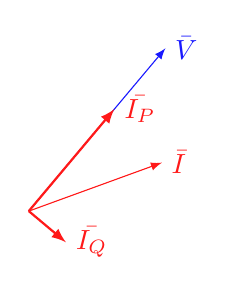
\begin{tikzpicture}[scale=1, samples=100, >=latex]
	\def\Theta{50}
	\def\Phase{-30}
	\def\VoltageMagnitude{2.7}
	\def\CurrentMagnitude{1.8}
	\def\IpMagnitude{1.6914}	
	\def\IqMagnitude{0.6156}	
	\def\c{{\VoltageMagnitude*sin(\Theta)}}
	\def\StromWert{{\CurrentMagnitude*sin(\Theta+\Phase)}}
	%%%%%%%%%%%%%%%%%%%%%%%%%%%%%%%%%%%%%%%%%%%%%%%%%%%%%%%%%%
	\def\VoltageColor{blue!90!white}
	\def\CurrentColor{red!90!white}
	\def\FarbeWinkelZeichnung{\VoltageColor}
	%%%%%%%%%%%%%%%%%%%%%%%%%%%%%%%%%%%%%%%%%%%%%%%%%%%%%%%%%%
	\def\Beta{\Theta+\Phase}
	\def\ThetaRad{\Theta*3.141592654/180}
	\def\PhaseRad{\Phase*3.141592654/180}
	%%%%%%%%%%%%%%%%%%%%%%%%%%%%%%%%%%%%%%%%%%%%%%%%%%%%%%%%%%
	% voltage angle 
	%\filldraw[fill=\FarbeWinkelZeichnung!20,draw=\FarbeWinkelZeichnung!50!black] (0,0) -- (1,0) node[above=5pt, color = \VoltageColor] {$\theta$} arc (0:\Theta:1) -- cycle; 
	% Current angle
	%\filldraw[fill=\CurrentColor!20,draw=\CurrentColor!50!black] (0,0)  -- (0.7,0) node[above,  color = \CurrentColor] {$\psi$} arc (0:\Beta:0.7) -- cycle ;
	% Display axes
	%\PlotAxesWithoutLabels{0}{3}{-1.6}{2.6}{0}
	
	% voltage pointer
	\draw[->,color=\VoltageColor] (0,0) -- (\Theta:\VoltageMagnitude) node[right]{$\bar{V}$};
	
	% current pointer
	\draw[->,color=\CurrentColor] (0,0) -- (\Beta:\CurrentMagnitude) node[right]{$\bar{I}$};
	
	% Active current pointer
	\draw[->,color=\CurrentColor,  thick] (0,0) -- (\Theta:\IpMagnitude) node[right]{$\bar{I_P}$};
	
	% Active current pointer
	\draw[->,color=\CurrentColor,  thick] (0,0) -- (-40:\IqMagnitude) node[right]{$\bar{I_Q}$};
	
	
	\end{tikzpicture}
}

